\section{Acceso al sistema}

\subsection{Ingreso a Odoo Online}

\begin{itemize}
    \item \textbf{URL de la instancia:} \href{https://machu-picchu-exclusive-tours.odoo.com/odoo}{\texttt{https://machu-picchu-exclusive-tours.odoo.com/odoo}} (acceso web a Odoo Online de Machu Picchu Exclusive Tours).
    \item \textbf{Usuario (e-mail de ingreso):} \href{mailto:machupicchuexclusive.tours.eirl@gmail.com}{\texttt{machupicchuexclusive.tours.eirl@gmail.com}}. Cada persona debe usar su propio acceso; no comparta credenciales.
    \item \textbf{Contraseña:} se entrega \textbf{por un canal privado} acordado con la gerencia o el equipo consultor (no se consigna en este manual por seguridad). Tras recibirla, considere una contraseña robusta y, si la política de la empresa lo permite, active la verificación en dos pasos ofrecida por Odoo.
\end{itemize}

Tras el primer acceso, confirme en \textbf{Preferencias} (menú del usuario, arriba a la derecha) que el \textbf{idioma de la interfaz} sea \textbf{Español (Latinoamérica)} o el español que utilice su equipo, y que la \textbf{zona horaria} corresponda a la operación (por ejemplo Lima). La instancia está configurada con \textbf{una sola moneda de trabajo: dólares estadounidenses (USD)}.

\subsection{Moneda y cotizaciones (sin impuestos)}

En el catálogo y en las cotizaciones u órdenes, los importes se manejan en \textbf{USD} y se presentan \textbf{sin impuestos} (montos netos, sin IGV ni otros tributos sumados en pantalla o en el PDF según la parametrización acordada). Cualquier obligación tributaria o tratamiento contable externo se gestiona fuera de este flujo operativo cotidiano en Odoo; ante duda, consulte al asesor contable de la empresa.

\subsection{Pantalla inicial y menú de aplicaciones}

La pantalla principal de Odoo organiza el trabajo por \textbf{aplicaciones} (CRM, Proyectos, Ventas, etc.). Desde el menú de aplicaciones puede fijar en favoritos los módulos de uso diario. Si no ve alguna aplicación, puede deberse a permisos de usuario: solicite al administrador el perfil adecuado.

\begin{figure}[H]
    \centering
    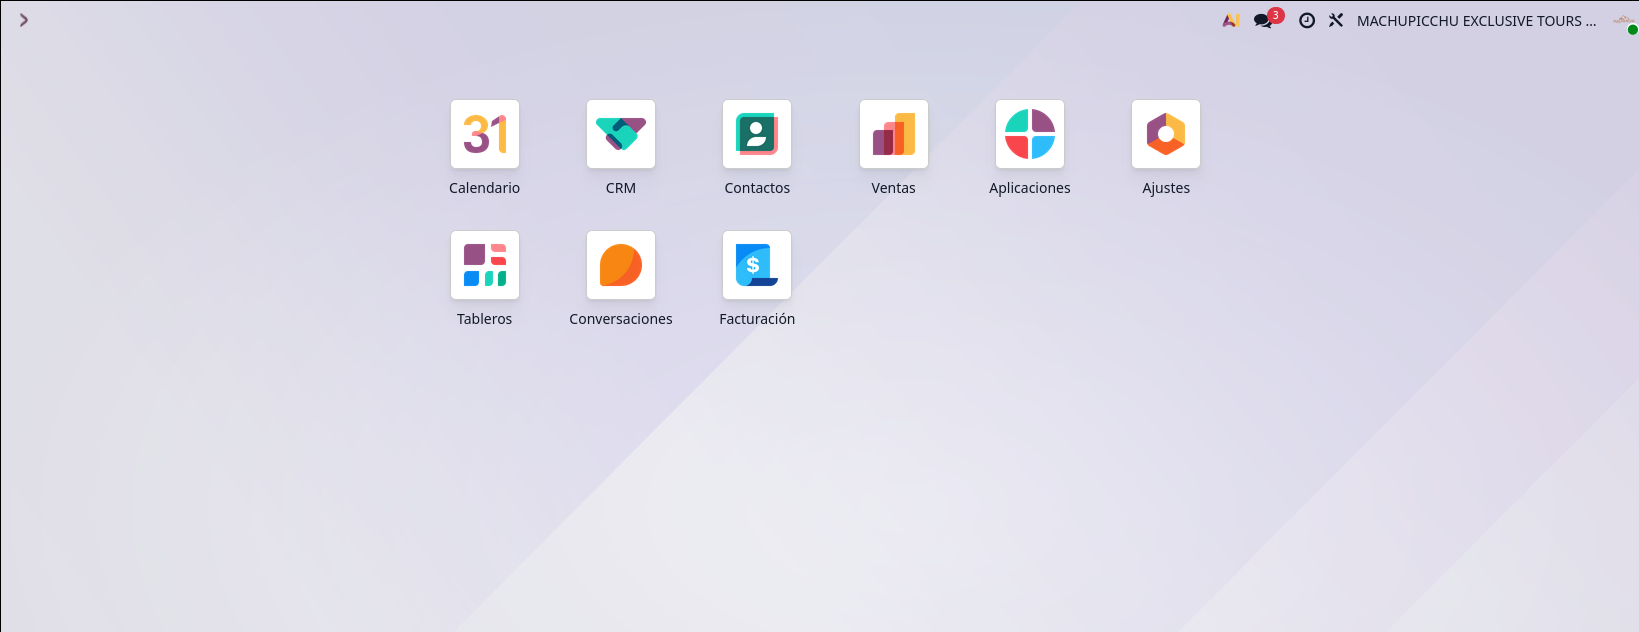
\includegraphics[width=0.95\textwidth]{assets/odoo-pantalla-principal-menu-aplicaciones.png}
    \caption{Pantalla principal de la instancia Odoo Online (menú de aplicaciones), Machu Picchu Exclusive Tours}
\end{figure}

\subsection{Buenas prácticas de seguridad}

\begin{itemize}
    \item Centralice documentos sensibles (pasaportes, identificación) en la \textbf{ficha del cliente} según lo acordado en implementación; reduzca el intercambio por canales personales sin respaldo institucional.
    \item Evite almacenar ``copias paralelas'' definitivas solo en equipos personales; use Odoo como \textbf{fuente de verdad} operativa.
\end{itemize}
